% ============================================================
% Classic RL agent-environment loop
% Compile with:  pdflatex rl_agent_loop.tex
% Output:        rl_agent_loop.pdf
% ============================================================
\documentclass[border=4pt]{standalone}
\usepackage{tikz}
\usetikzlibrary{shapes.geometric, arrows.meta, positioning, fit, backgrounds, calc}

\definecolor{colAgent}{RGB}{220,235,245}
\definecolor{colEnv}{RGB}{220,245,220}
\definecolor{colBorder}{RGB}{80,100,120}
\definecolor{colArrow}{RGB}{60,80,100}

\tikzset{
  box/.style={
    rectangle, rounded corners=3pt,
    draw=colBorder, line width=0.7pt,
    text centered, font=\small,
    inner sep=5pt, minimum height=1.8em
  },
  agentBox/.style={
    box, fill=colAgent,
    minimum width=3.2cm, minimum height=2.0cm,
    align=center
  },
  envBox/.style={
    box, fill=colEnv,
    minimum width=3.2cm, minimum height=2.0cm,
    align=center
  },
  arr/.style={
    -{Stealth[length=5pt]}, line width=0.8pt, color=colArrow
  },
  label/.style={
    font=\small, text=colBorder
  }
}

\begin{document}
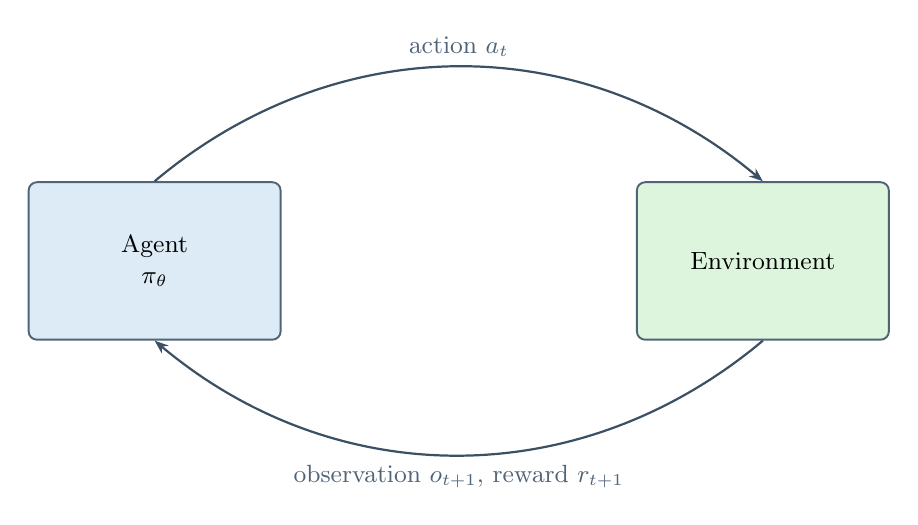
\begin{tikzpicture}[node distance=4.5cm]

  \node[agentBox] (agent) {Agent\\$\pi_\theta$};
  \node[envBox, right=of agent] (env) {Environment};

  % action arrow (top): agent -> env
  \draw[arr] (agent.north) to[bend left=40] node[label, above] {action $a_t$} (env.north);

  % observation + reward arrow (bottom): env -> agent
  \draw[arr] (env.south) to[bend left=40] node[label, below] {observation $o_{t+1}$, reward $r_{t+1}$} (agent.south);

\end{tikzpicture}
\end{document}
